\chapter*{Introducción}\label{chapter:introduction}
\addcontentsline{toc}{chapter}{Introducción}

Resulta común que la actividad de los gobiernos nacionales genere déficits 
continuados en los balances presupuestarios anuales, por lo que se emplean mecanismos de financiación adicionales a las fuentes convencionales de 
ingresos fiscales. En este sentido, se reconocen dos vías para la financiación pública: 
la monetización  y los mecanismos de mercado a partir de una política de endeudamiento público. 
La experiencia negativa de un numeroso grupo de países con relación a los efectos de 
la monetización sobre la inflación generó un rechazo prácticamente rotundo a esta 
alternativa, concentrando la financiación del gobierno en el endeudamiento soberano. 

En la actualidad ambos tipos de financiamiento ocurren en los Mercados de Deuda 
Pública (MDP). 
El MDP es un mercado financiero que cuenta con dos segmentos o submercados: el 
primario y el secundario. En el primero de ellos se emiten y colocan inicialmente los 
títulos de deuda del gobierno, y en el segundo, estos valores se transan continuamente 
hasta su vencimiento. Es el espacio, no necesariamente físico, donde se comercializan 
los valores del gobierno y donde éste obtiene financiamiento de diversos agentes. 

En Cuba, durante más de 40 años los déficits fiscales fueron monetizados 
íntegramente, en una primera etapa por el Banco Nacional de Cuba (BNC) y luego por 
el Banco Central de Cuba (como prestamista de única instancia), sin el establecimiento 
de un compromiso explícito de amortización. 
Si bien en los años más recientes la monetización en el país no se ha traducido en un impacto directo sobre los precios, dadas las características peculiares de la economía 
doméstica, su empleo a lo largo del tiempo ha generado otras distorsiones. 
A raíz del proceso de actualización del modelo económico iniciado con el VI Congreso 
del Partido Comunista de Cuba y en particular, del reordenamiento del entorno económico, monetario y financiero, se comenzaron a gestar e implementar un conjunto de transformaciones en los mecanismos para financiar al Presupuesto del Estado. Este proceso ha estado apoyado en la intención institucional de crear a mediano plazo un Mercado de Deuda Pública. 

En un futuro escenario de ese tipo, el Estado cubano pide dinero prestado a entidades de la econom\'ia a trav\'es del Banco Central de Cuba. El monto solicitado y el inter\'es m\'aximo con el que se devolver\'a se plasman en un documento llamado bono soberano.  Los posibles prestamistas participan en una subasta por el bono y el que menor tasa de inter\'es exija por el pr\'estamo ser\'a el ganador, y el Estado pasar\'a a ser su prestatario.  

Para decidir qui\'enes participan en la subasta, se confeccionan los Comit\'es de Mercado Financiero (CMF).  El Comité de Mercados Financieros (CMF) del BCC es la Autoridad de Mercado (AM) que regirá el reglamento del MDP. Podrá adoptar todas aquellas medidas que juzgue convenientes para la estabilidad y desarrollo del mercado, y tendrá potestad disciplinaria sobre todos los Operadores del Mercado, cualquiera sea su clase o naturaleza. Los miembros y el presidente de cada Comit\'e se deciden mediante un proceso electoral en el que cualquier elector puede ceder su poder de voto a otro elector. A ese tipo de elecci\'on el autor le denomina \textbf{votaci\'on representativa}.  


En un sistema de votaci\'on representativa  los votos se transfieren, esto es, si una persona $A$ vota por una persona $B$ y esta, a su vez, vota por  $C$, entonces el voto de $A$ se transfiere a $C$. Luego, cada participante puede ser a la vez votante y candidato. Formalmente, el c\'alculo de los votos obtenidos por un candidato puede ser definido recursivamente de la siguiente manera:
\begin{equation}\label{eq:votes-count}
    \#_{votos}(y) = \begin{cases}
        |V_y| + \underset{x \in V_y}{\sum} \#_{votos}(x) & \text{si } V_y \neq \emptyset \\
        0 & \text{si } V_y = \emptyset 
    \end{cases}
\end{equation}
donde $V_y$ es el conjunto de personas que votaron directamente por $y$. La figura~\ref{fig:r-voting} ilustra un ejemplo de votación en el que $A$ votó por $B$, $B$ y $E$ votaron por $C$ y $C$ votó por $D$. $B$ obtiene solamente el voto de $A$, mientras que $C$ obtiene los votos de $A$, $B$ y $E$. $D$ recibe el voto directo de $C$ y, con este,  los votos indirectos de los restantes participantes. Cerca de cada flecha se encuentra un n\'umero que indica la cantidad de votos que se transfieren. Encima de cada candidato se encuentra el n\'umero de votos que obtiene.

\begin{figure}[h!]
    \centering
    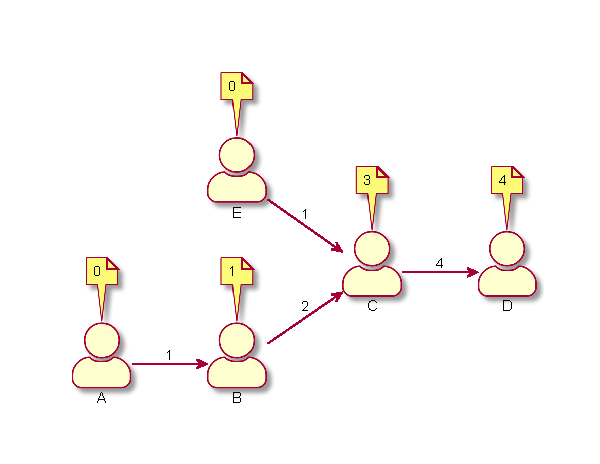
\includegraphics{Graphics/rep-voting.pdf}
    \caption{Conteo de votos en votación representativa.}
    \label{fig:r-voting}
\end{figure}

\todo[disable,inline]{@FIXME ba'jales la altura al pdf generado de las figuras~\ref{fig:r-voting}~y~\ref{fig:voting-cycle}}

En el caso particular de la confecci\'on de los CMF, cada individuo puede votar por a lo sumo otra persona.



En un proceso electoral de este tipo pueden surgir ciclos de votación, como el que se muestra en la figura~\ref{fig:voting-cycle}, donde el voto emitido por $D$ hacia $B$ forma un ciclo que los involucra a ambos y a $C$.  

\begin{figure}[h!]
    \centering
    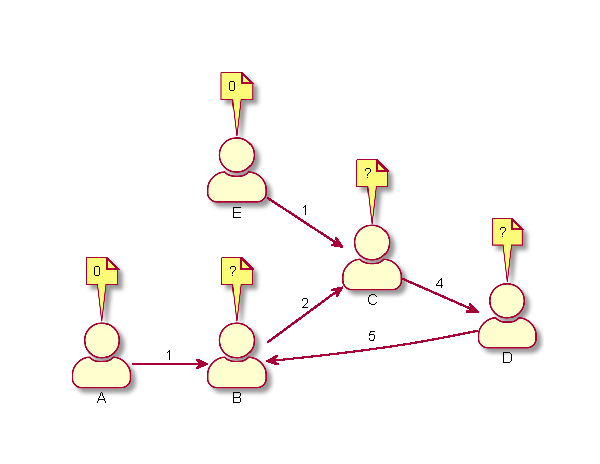
\includegraphics{Graphics/voting-cycle.pdf}
    \caption{Ciclo de votaci\'on.}
    \label{fig:voting-cycle}
\end{figure}


En un  caso como ese, no se puede aplicar sin m\'as la f\'ormula~\eqref{eq:votes-count} para calcular los votos obtenidos por los candidatos involucrados en el ciclo.  La naturaleza recursiva de $\#_{votos}$ impide su c\'alculo en ciclos de votaci\'on, debido a la ocurrencia de dependencias circulares. Por ejemplo, en la figura~\ref{fig:voting-cycle} se puede apreciar que el c\'alculo de los votos que $C$ obtiene depende del c\'alculo de los votos de $B$, y este, a su vez, depende del valor de $\#_{votos}(D)$, pero $D$ depende del n\'umero de votos obtenidos por $C$. Se forma entonces un c\'irculo de dependencias y no puede ser calculado apropiadamente el n\'umero de votos obtenido por cada uno de los candidatos $B$, $C$ y $D$.



% pa mantener un sistema distribuido de goquorum es necesario al menos 4 nodos % @NOTE chekea eso 

Tradicionalmente en estas elecciones, como en muchas otras, los votos son emitidos en boletas de papel y el conteo es realizado manualmente. Esto puede traer consigo ciertos problemas que causan desconfianza en el electorado, como son los votos falsos y el mal conteo de los votos.   Si no se hace una verificaci\'on rigurosa de la identidad del votante, entonces se puede emitir votos con relativa facilidad en nombre de personas que no han votado (votos falsos). Si el conteo no est\'a supervisado adecuadamente, pueden surgir errores en los resultados, ya sea por intereses personales o errores humanos.

En un sistema de votaci\'on electr\'onico se  pueden lograr diversas formas de verificaci\'on biom\'etrica, por ejemplo, mediante la huella digital o el esc\'aner ocular. Por otro lado, en estos sistemas se puede contar los votos de manera eficiente mientras se van realizando y se  puede publicar en vivo los resultados. 

Otras bondades poseen los sistemas electrónicos, como son la flexibilidad, lo fácil que pueden ser de usar y lo baratos que resultan con respecto a los sistemas tradicionales. Sin embargo, muchos de los sistemas electrónicos existentes son centralizados, esto es, dependen de que una agencia central se encargue de registrar, manejar, calcular y revisar los votos. Toda la confianza debe entonces ser depositada en esa agencia, lo cual hace vulnerable al sistema.
 
Un sistema digital descentralizado de votación no tiene ese problema. Una de las tecnologías descentralizadas empleadas actualmente es \textit{blockchain}.   \textit{Blockchain} es un registro distribuido e inmutable  de transacciones. Lo que se transacciona puede ser tangible, como son  una casa o dinero en efectivo, o intangible, como son el derecho de autor de una obra o el voto de un elector por un candidato (\cite{blockchain-ibm}). La inmutabilidad y seguridad de este registro se basan en principios de  criptografía, descentralizaci\'on y mecanismos de consenso (\cite{blockch-security-ibm}). 


% Hacerlo con \textit{blockchain} ta bueno xq resuelve la parte m\'as importante de esos problemas. 

Desde el surgimiento de Ethereum se puede implementar comportamientos complejos mediante contratos inteligentes. Ethereum es una plataforma \textit{blockchain} que establece una red p\'ublica que ejecuta y verifica c\'odigo de manera segura. A dicho c\'odigo o al programa que resulta de ejecutarlo se le conoce como contrato inteligente (\cite{eth-aws}).  

No es deseable que el proceso electoral en el CMF se realice en una red p\'ublica, ya que es un proceso que s\'olo concierne a las partes involucradas. Por otro lado, desplegar un contrato inteligente en Ethereum puede costar miles de d\'olares (\cite{eth-deploy}). Estos dos factores hacen que no sea factible realizar la implementaci\'on de este trabajo sobre la red p\'ublica de Ethereum. 

GoQuorum es una implementaci\'on de Ethereum capaz de crear redes privadas y con mecanismos de autorizaci\'on. En GoQuorum tambi\'en se puede personalizar el costo del despliegue de los contratos inteligentes, incluso, puede hacerse nulo. Por todo lo dicho anteriormente, GoQuorum es una buena opci\'on en la que implementar el sistema de votaci\'on representativa del CMF.


Existen implementaciones de sistemas de votaci\'on en otras \textit{blockchain} (\cite{agora}) y tambi\'en en Ethereum (\cite{ovn} y \cite{borda_count}), pero no se conoce ninguna implementaci\'on de un sistema de voto representativo en GoQuorum.

El sistema a implementar debe cumplir los siguientes requisitos:
\begin{itemize}
    \item ser capaz de calcular los votos siguiendo la f\'ormula~\eqref{eq:votes-count}, teniendo en cuenta la ocurrencia de ciclos;
    \item obtener un \'unico ganador como resultado de las elecciones;
    \item que pueda ser desplegado sobre una red GoQuorum;
    \item contar correctamente todos los votos v\'alidos e ignorar los votos inv\'alidos;
    \item prevenir que sean registrados dos votos distintos a nombre del mismo votante;
    \item permitir votar a s\'olo los votantes registrados.
\end{itemize}

\todo[inline, disable]{@TODO decir que el Instituto de Criptograf\'ia implement\'o un sistema de votaci\'on en hyperledger fabric pero tampoco nos sirve. ?`C\'omo cito eso?}

El presente trabajo de diploma   debe responder a la interrogante: ?`c\'omo dise\~nar un sistema de votaci\'on electr\'onico que cumpla con los requisitos mencionados anteriormente? Para ello deben lograrse ciertos objetivos, a saber: dise\~nar algoritmos que satisfagan los requerimientos,  implementarlos en forma de contratos inteligentes y evaluarlos en una red privada de GoQuorum.

A continuaci\'on se enumeran las tareas que deben ser realizadas para lograr los objetivos mencionados:
\begin{enumerate}
    \item realizar una revisi\'on de la bibliograf\'ia existente acerca de sistemas de votaci\'on electr\'onico sobre \textit{blockchain}, as\'i como de los sistemas electorales que se utilizan en la actualidad y sus mecanismos de desempate;
    \item valorar los resultados de la revisi\'on anterior;
    \item dise\~nar algoritmos que permitan contar y desempatar apropiadamente;
    \item estudiar el lenguaje de programaci\'on Solidity;
    \item implementar los contratos inteligentes que sean necesarios;
    \item evaluar esos contratos.
\end{enumerate}

\todo[inline,disable]{@TODO decir d q' va cada capi'tulo}

% @NOTE habla en tiempo presente, 3ra persona del singular, e.g. "el autor ha desarrollado", "el autor ha realizado", etc.

\todo[inline,disable]{@TODO usa \textbackslash citep o el ekivalente cuan2 usas babel cuan2 citas adentro d pare'ntesis. Trae opcio'n pa citas mu'ltiples}